\chapter{Large scale solar power plants}
%Almost all power that we use on our planet comes from the sun. Direct in form of radiation or indirect during wind, water and vegetation. Also the fossil power resources and reserves are stored energy from the sun in from of organic carbon compounds. There are two main technologies for generating electricity out of direct sun radiation. One is the direct conversion of solar irradiance to electrical energy while using photovoltaic. The other is to generate heat and convert it to electrical power. Figure~\ref{OverviewSTP} gives an abstract of the common technologies using direct solar power to generating electric power. This chapter has the focus on large-scale solar power plants and describes parts from both technologies.
Virtually all energy consumed on Earth comes from the sun, whether directly in the form of solar radiation, or indirectly through wind, the water cycle or vegetation. Even the energy in fossil fuels is simply solar energy stored in the form of organic carbon compounds. There are two main technologies for generating electricity out of direct solar radiation. One is the direct conversion of solar irradiance to electrical energy via the photovoltaic effect. The other is to first convert that solar irradiance heat and use that heat to generate electricity. Figure~\ref{OverviewSTP} graphically shows the relationships between common solar technologies for generating generating electric power. The technologies which are the focus of this work are highlighted in red.

\begin{figure}[!h] 
\centering
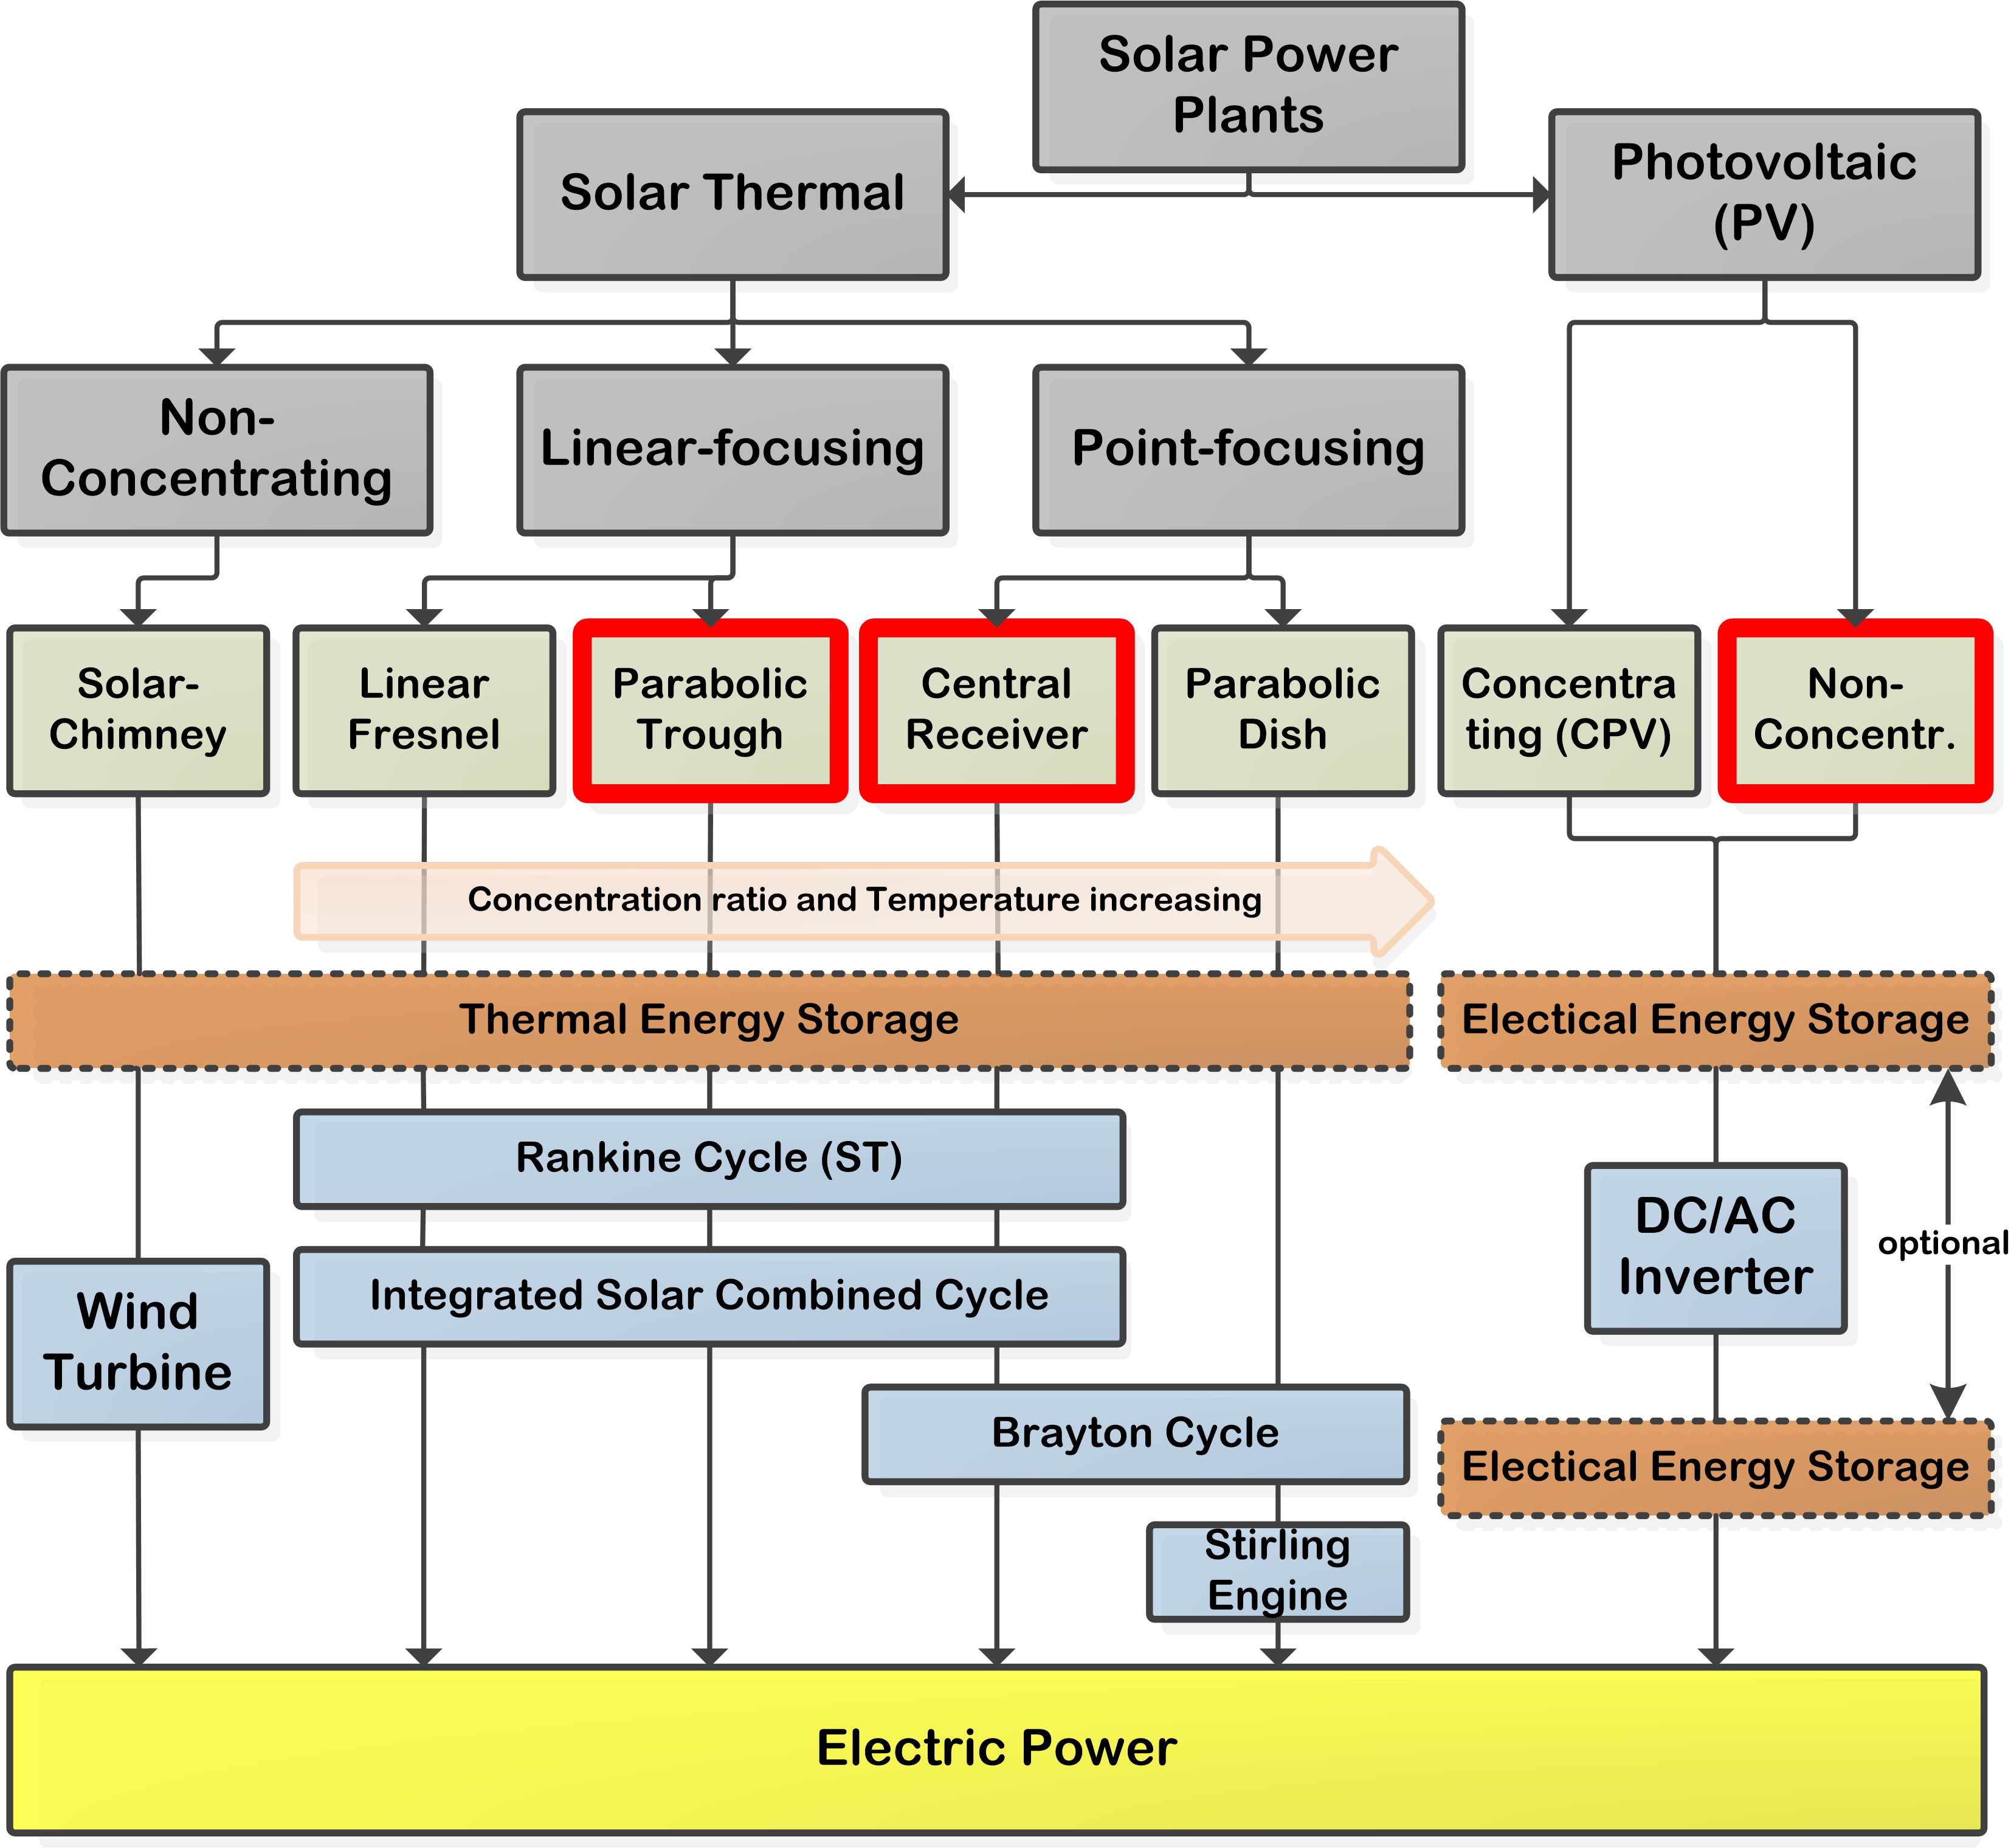
\includegraphics[width=0.75\linewidth]{FIG/OverviewSTP}
\caption[Overview of Solar Power Technologies.]{Overview of Solar Power Technologies.}\label{OverviewSTP}
\end{figure}


%Therefore it is split in the technology fields of large scale concentrated solar power plants (\ref{Large scale concentrated solar power (CSP) plants}) and large scale photo voltaic power plants (\ref{Large scale photo voltaic (PV) power plants}).
%In detail the technologies with a large-scale power plant potential -- parabolic trough, central receiver and non-concentrating photovoltaic -- are described. Also the storage systems for both systems. 
%Therefore it is split in the technology fields of large scale concentrated solar power plants (\ref{Large scale concentrated solar power (CSP) plants}) and large scale photo voltaic power plants (\ref{Large scale photo voltaic (PV) power plants}).
%In detail the technologies with a large-scale power plant potential -- parabolic trough, central receiver and non-concentrating photovoltaic -- are described. Also the storage systems for both systems. 

\section{Large-scale CSP plants}\label{Large scale concentrated solar power (CSP) plants}
%Concentrating solar power (CSP) systems use combinations of mirrors or lenses to concentrate direct beam solar radiation to produce forms of useful energy such as heat, electricity and others. This happens by use of various downstream technologies. Generally the CSP technology includes not only the concentrating solar thermal (CST) technology, but also concentrating photovoltaic (CPV) energy conversion. However, there is no focus on CPV in this thesis. That is why the term CST is put on a level with CSP.
Concentrating solar power (CSP) systems use combinations of mirrors or lenses to concentrate direct beam solar radiation to produce forms of useful energy such as heat and electricity. This happens by use of various downstream technologies. Generally, CSP technology includes not only concentrating solar thermal (CST) technology, but also concentrating photovoltaic (CPV) energy conversion. However, CPV will not be treated in this thesis.
%A CSP plant comprises four main sub-systems: concentrating system, solar receiver, storage and power block. Also supplementary firing is used in some cases, but is basically not necessary nowadays. A graphic scheme of such a sub-system is shown in Figure~\ref{MainComp}. The separate components are linked together by energy flow in mostly radiation transfer or fluid transport. This chapter describes the function and gives an application overview of the individually components. 
A CSP plant comprises four main sub-systems: concentrating system, solar receiver, storage and power block (Figure~\ref{MainComp}). (Supplementary firing was used in the past, but is not necessary nowadays.) The separate components are energetically linked via radiation or fluid transport.
\begin{figure}[!h] 
\centering
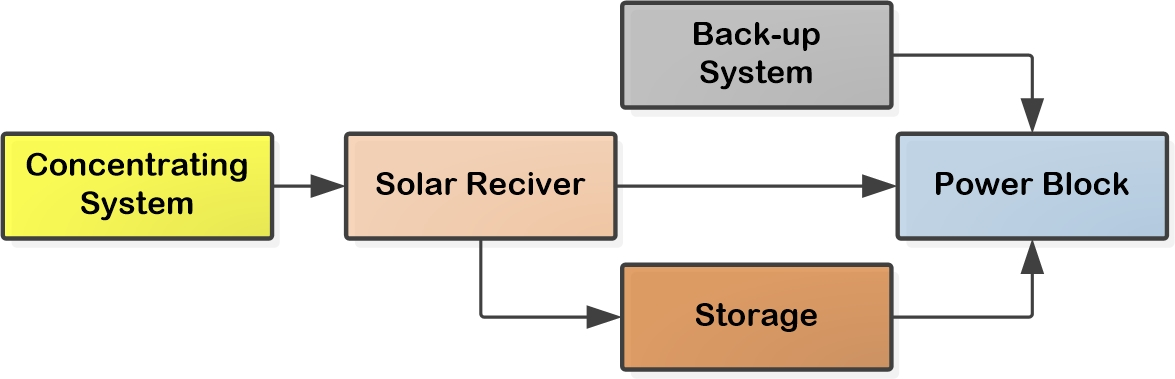
\includegraphics[width=0.85\linewidth]{FIG/MainComp}
\caption[Main components of a CSP plant.]{Main components of a CSP plant.}\label{MainComp}
\end{figure}

%The main advantage of CSP in opposite to other renewable energy producers is the thermal storage to provide power for cloudy days or during night time. Therefore the concentrating system and solar receiver have to produce more thermal energy then the power block can use directly. The ratio of the power capacity of the collector field to the capacity of the power block is defined as Solar multiple (SM). For CSP systems with storage, the number of hours of storage is based on the capacity of the power block. Chapter \ref{Subsection_storage_system} describes technical possibilities and application of thermal storage system for CSP.
The main advantage of CSP when compared to other renewable energy producers is its thermal storage, which continues to provide power on cloudy days at night. This means that the concentrating system and solar receiver must produce more thermal energy then the power block can use directly. The ratio of the output of the collector field to the output of the power block is defined as \emph{solar multiple} (SM). For CSP systems with storage, the number of hours of storage is based on the capacity of the power block (Chapter \ref{Subsection_storage_system} describes technical aspects and applications of thermal storage systems in CSP).

%The solar receiver or concentrating system is eponymously for the main CST technologies. The two most common CSP plant technologies are parabolic trough collector (PTC) and central receiver (CR) systems (also known as solar power towers). Further types of CSP plant are linear Fresnel reflectors (LFR) and parabolic dish. The main difference of the technologies is the concentrating system. Thereof results the differences in optical design, shape of receiver, nature of the transfer fluid and capability to store heat before it is turned into electricity. In systems with a line focus (PTC trough and LFR) the mirrors track the sun along one axis. In those with a point focus (CR and parabolic dish), the mirrors track the sun along two axes. The receiver may be fixed, as in LFR and CR, or mobile as in PTC and parabolic dish systems. An overview of the technologies and there differences in relation to the focus and the receiver  is shown in Table \ref{tbl: CSPtech}.
The two most common CSP plant technologies are parabolic trough collector (PTC) and central receiver (CR) systems (also known as solar power towers). Other types include linear Fresnel reflector (LFR) and parabolic dish. The main difference between these technologies is the concentrating system, which lead to differences in optical design, shape of receiver, nature of the transfer fluid and capability to store heat before it is turned into electricity. In systems with a line focus (PTC and LFR) the mirrors track the sun along one axis. In those with a point focus (CR and parabolic dish), the mirrors track the sun along two axes. The receiver may be fixed, as in LFR and CR, or mobile as in PTC and parabolic dish systems (see Table \ref{tbl: CSPtech}).

\begin{table}[h!] % Main technologies 
  \centering
  \begin{tabular}{  m{5cm}  m{5cm}  m{5cm}  }
    \hline
    & \textbf{Line focus} & \textbf{Point focus} \\ 
    & Collectors track the sun along a single axis and focus irradiance on a linear receiver. This makes tracking the sun simpler. & Collectors track the sun along two axes and focus irradiance at a single point receiver. This allows for good receiver efficiency at higher temperatures.\\ \hline \hline
    \textbf{Fixed receiver} & &\\

    Fixed receivers are stationary devices that remain independent of the plant's focusing device. This eases the transport of collected heat to the power block.
    &
    \begin{minipage}[t]{5cm}
      \centering
	 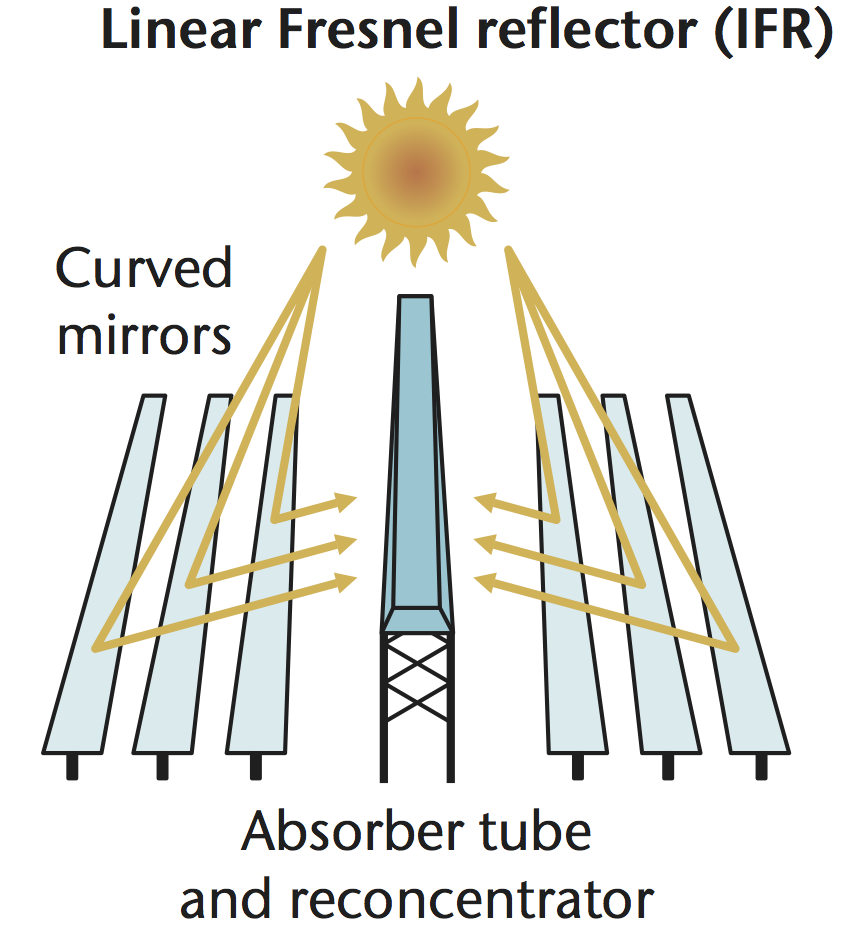
\includegraphics[height=55mm]{FIG/SUM/LF}
    \end{minipage}
    & 
    \begin{minipage}[t]{5cm}
      \centering
	  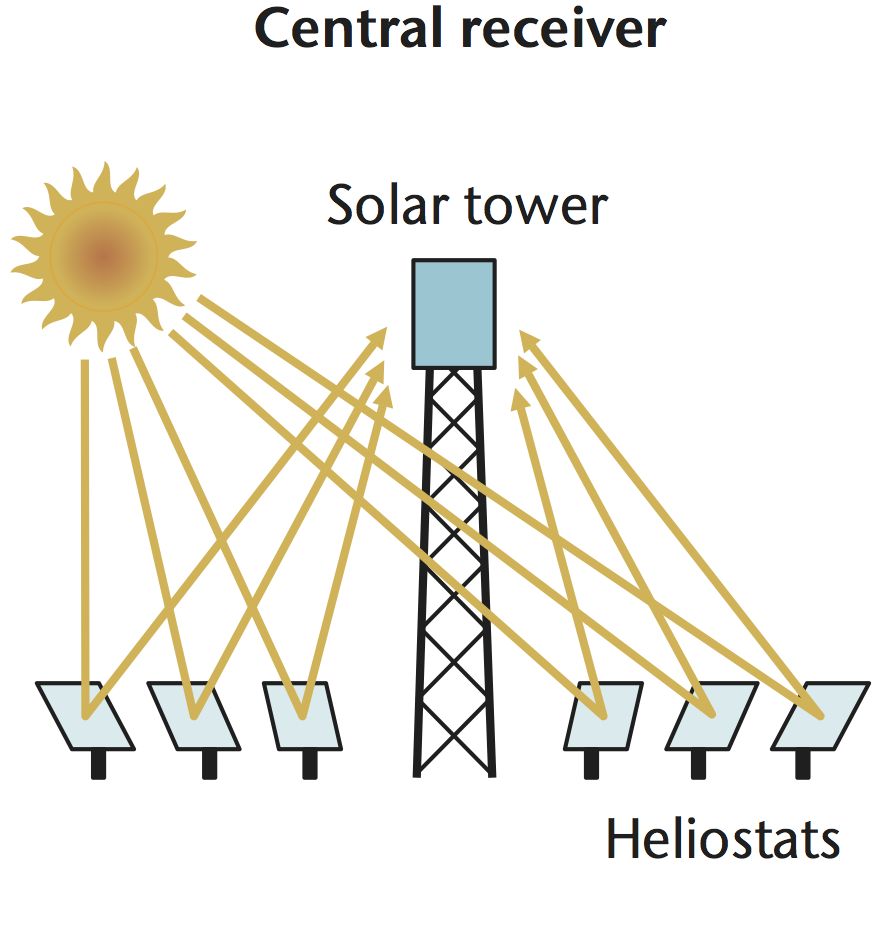
\includegraphics[height=55mm]{FIG/SUM/ST}
    \end{minipage}
    \\ \hline
    \textbf{Mobile receiver} & & \\
    Mobile receivers move together with the focusing device. In both line focus and point focus designs, mobile receivers collect more energy.
    &
    \begin{minipage}{5cm}
      \centering
	  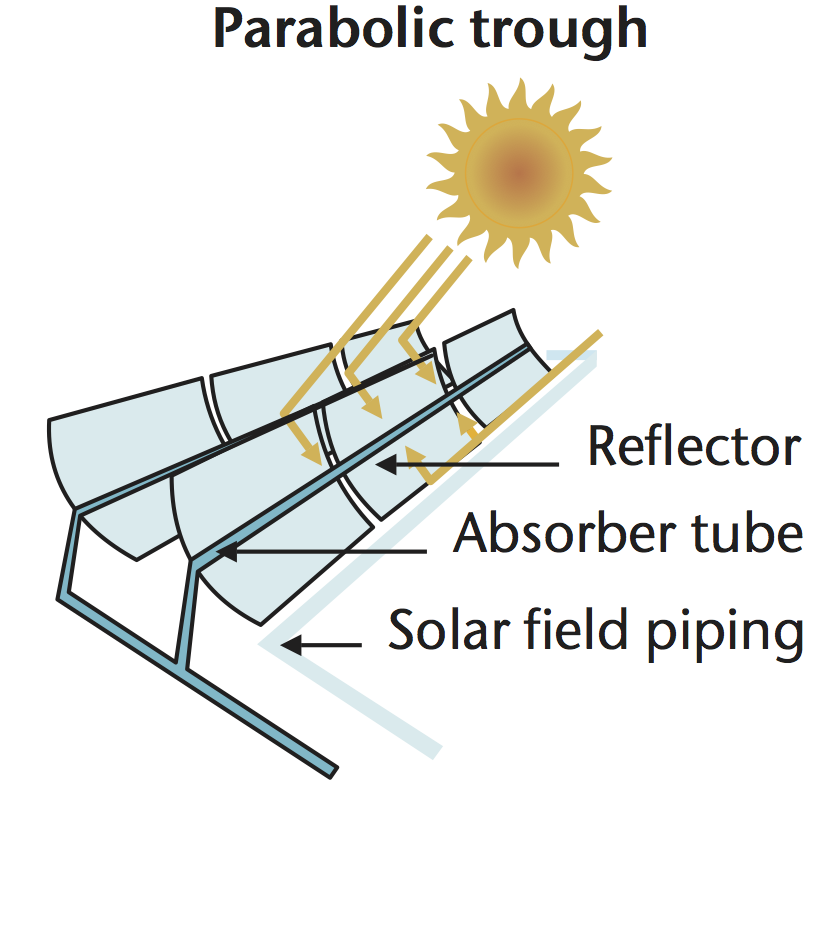
\includegraphics[height=55mm]{FIG/SUM/PT}
    \end{minipage}
    & 
    \begin{minipage}{5cm}
      \centering
	  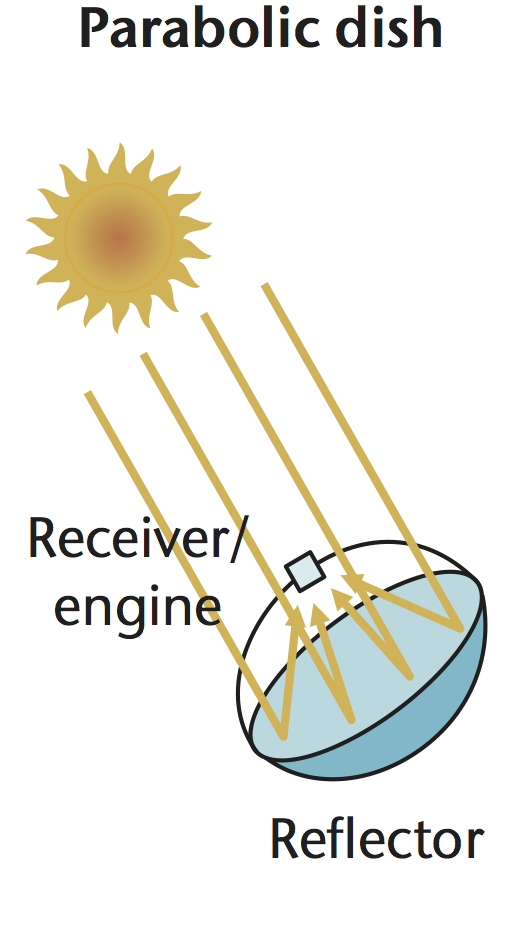
\includegraphics[height=55mm]{FIG/SUM/PD}
    \end{minipage}    
    \\ \hline
  \end{tabular}
  \caption[CSP technology families.]{CSP technology families \cite{IEA2014b}.}\label{tbl: CSPtech}
\end{table}


%As mentioned above is main difference between the CSP technology families how they concentrate the solar radiation. This strongly affects their overall efficiency. The parabolic dish has the best annual optical efficiency (about 90\%) because the concentrator axis is always parallel to the sun rays. The worst (about 50\%) is observed for linear Fresnel systems because of poor performance in the morning and in the evening. Intermediate values (65-75\%) are obtained for parabolic trough and tower systems. For each family the actual efficiency varies with the location, the time of day and the season of the year. \cite{EASAC2011} 
The main difference between the CSP technology families is in how they concentrate the solar radiation, which affects their overall efficiency. The parabolic dish has the best annual optical efficiency (\~\SI{90}{\percent}) because the concentrator axis is always parallel to the sun's rays. The worst (\~\SI{50}{\percent}) is observed for linear Fresnel systems because of poor performance in the morning and in the evening. Intermediate efficiencies (\SIrange{65}{75}{\percent}) are obtained for parabolic trough and central receiver systems. For each family, actual efficiency varies with location, time of day and season \cite{EASAC2011}.

%The capacity range of an CSP-plant is also strongly affected by the concentration ratio. The most common definition of concentration ratio is the ratio of the area of reflector aperture ($A_a$) to the area of receiver ($A_r$). The area concentration is:
The capacity range of a CSP plant is also strongly affected by the concentration ratio, which is defined as the ratio of the area of reflector aperture ($A_a$) to the area of receiver ($A_r$):

\begin{align}
C=\frac{A_{a}}{A_{r}} \label{GL_concentration}
\end{align}
%The concentration ratio from Equation \ref{GL_concentration} has an upper limit that depends on whether the concentration is a three dimensional (point focus) concentrator such as a parabolic dish and central receiver solar tower or a two-dimensional (linear focus) concentrator such as parabolic trough and linear Fresnel reflector. The maximum concentration ratio is based on the second law of thermodynamics applied to radiative heat exchange between the sun and the receiver. The maximum possible concentration ratio for circular concentrators is 45~000, and for linear concentrators is the maximum 212. \cite{Duffie2013}
The concentration ratio from Equation \ref{GL_concentration} has an upper limit that depends on whether the concentration is a three-dimensional (point focus) concentrator such as a parabolic dish or central receiver, or a two-dimensional (linear focus) concentrator such as a parabolic trough or linear Fresnel reflector. The maximum concentration ratio is based on the second law of thermodynamics applied to radiative heat exchange between the sun and the receiver. The maximum possible concentration ratio for circular concentrators is \num{45000}, for linear concentrators it is \num{212} \cite{Duffie2013}.

\begin{table}[h!]  
  \centering
	\begin{tabular}{  p{3.0cm}  C{2.0cm}  C{2.2cm}  C{2.0cm}  C{2.0cm}  C{2.0cm}} 
\hline
\textbf{Technology} & \textbf{Capacity range} (\si{\mega\watt}) & \textbf{Concent- ration} & \textbf{Peak system efficiency} (\si{\percent}) & \textbf{Annual system efficiency} (\si{\percent}) & \textbf{Thermal cycle efficiency} (\si{\percent}) \\ \hline \hline
Parabolic trough & 10-280$^1$ & 70-100 & 21 & 10-16 & 35-42 ST  \\ \hline
Fresnel reflector & 10-200 & 25-100 & 20 & 9-13 & 30-42 ST  \\ \hline
Solar tower & 10-200 &  300-1~000 & 23 & 8-23 & 0-45 ST  \\ \hline
Dish-Stirling & 0.01-0.4 & 1~000-3~000 & 29 & 16-28 & 30-40  \\ \hline
\multicolumn{2}{l}{ST = Steam Turbine}
\end{tabular}
\caption[Performance characteristics CSP technology families.]{Performance characteristics CSP technology families \cite{Pitz-Paal.2013} \cite{AbengoaSolar2013a}$^1$.}\label{tbl: CSPCharacteristics}
\end{table}

%But actually the technical implementation of concentration ratio is the main parameter for the capacity range of a CSP plant. Table~\ref{tbl: CSPCharacteristics} gives an overview of some of the performance characteristics of the concentrating solar power concepts. More details are listed in Annexure I, Part A, Figure~\ref{CSPOverview1} on Page~\pageref{CSPOverview1} and Figure~\ref{CSPOverview2} on Page~\pageref{CSPOverview2}. PTC, LFR, and CR can be coupled to steam cycles of 10-280~MW electric capacity (and more), with thermal cycle efficiencies of 30-45~\%. Also the applies for stirling engines which are coupled to dish systems have similar efficiency ranges. The conversion efficiency of the power block remains essentially the same as in conventional-fired power plants. The annual system efficiency are the net power generation over incident beam radiation. They are lower than the conversion efficiencies of conventional steam or combined cycles, because they include the conversion of solar radiative energy to heat within the collector and the conversion of the heat to electricity in the power block. \cite{Pitz-Paal.2013}
% I do not understand the intended meaning of this sentence:
%But actually the technical implementation of concentration ratio is the main parameter for the capacity range of a CSP plant.

Table~\ref{tbl: CSPCharacteristics} gives an overview of performance characteristics (for further details, see Appendix I, Part A, Figure~\ref{CSPOverview1} on page~\pageref{CSPOverview1} and Figure~\ref{CSPOverview2} on page~\pageref{CSPOverview2}). PTC, LFR, and CR systems can be coupled to steam cycles of \SI{10280}{\mega\watt} electric capacity (and more), with thermal cycle efficiencies of \SIrange{30}{45}{\percent}. Stirling engines that are coupled to dish systems have similar efficiency ranges. The conversion efficiency of the power block is consistent with conventional power plants. The annual system efficiency is the net power generation over incident beam radiation. This is lower than the conversion efficiencies of conventional steam or combined cycles because it includes include the conversion of solar radiative energy to heat within the collector and the conversion of the heat to electricity in the power block \cite{Pitz-Paal.2013}.

\begin{figure}[!h] 
\centering
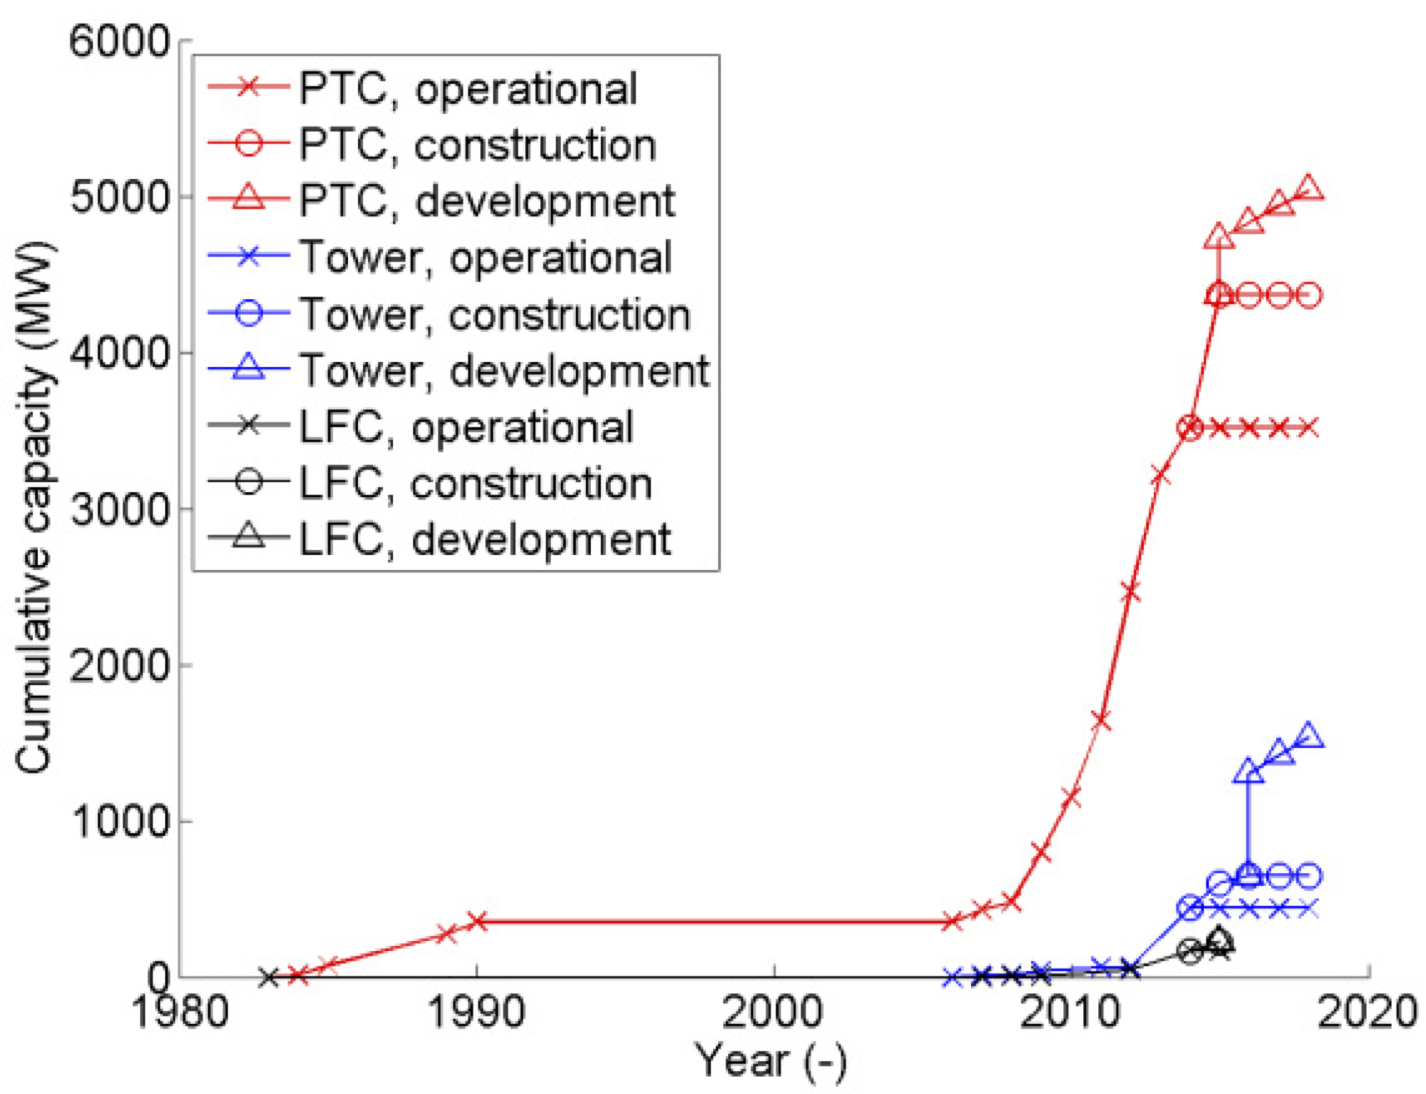
\includegraphics[width=0.65\linewidth]{FIG/CSP_technology_development}
\caption[Historical development of CSP technologies.]{Historical development of CSP technologies \cite{Abbas2015}.}\label{CSP_technology_development}
\end{figure}

%The development of the actual CSP plant technology goes back in the 1970's and 1980's, which is a consequent from the first two Oil crises. Figure~\ref{CSP_technology_development} shows the historical development of PTC, LFR in the Figure called linear Fresnel collector (LFC) and the CR (tower). The parabolic dishes have not succeeded at all and aren't shown here. The reason for that is mainly due to the high structural costs of moving an large diameter dish with two-axes tracking. One might observe that the predominant technology is the PTC, with an installed capacity well above 3~GW. CR have started the exponential development some years later compared to PTC, which explains why the operational installed capacity is much lower. Similarly the development for LFR have started even later, which drives to the lowest installed capacity of the three technologies. The difference in the timing of the three successful technologies is very influenced by the CSP development in its first golden period, the 1980's. In such period important central tower prototypes were built in USA (Solar One, Solar Two, CESA-1) and a 365~MW PTC solar plant was installed in the Mojave Desert. When the oil prices dropped at the end of the second oil crises interest on renewable energies was lost until the last decade. 
The development of the CSP technology began in earnest in the 1970s, a consequence of the first two oil price shocks. Figure~\ref{CSP_technology_development} shows the historical development of PTC and LFR (called linear Fresnel collector (LFC) here) technologies and the CR (tower). Parabolic dish systems have not been widely adopted and are not shown here; this is mainly due to the high costs associated with moving a large diameter dish with two-axis tracking. The predominant technology remains PTC, with an installed capacity well above \SI{3}{GW}. The development of central receiver systems began decades later, and that of linear Fresnel reflector systems later still; the operational installed capacity is proportional to the number of years the technology has been available. In the 1980s, important central tower prototypes were built in the USA (\emph{Solar One}, \emph{Solar Two}, \emph{CESA-1}) and the \SI{365}{\mega\watt} PTC solar plant was built at Kramer Junction in the Mojave Desert. When the oil prices dropped after the second oil crisis, interest in renewable energies was lost and it did not return until the beginning of the new millenium. 

%With regard to the past development in the different CSP technology dealt the following chapters with the PTC (\ref{subsection_PTC}) as well as with the solar tower technology (\ref{subsection_CRS}). The necessary concepts of the storage systems (\ref{Subsection_storage_system}) and an overview of common heat transfer fluids (\ref{subsection_HTF}) are also included. The systems for the converting thermal to electrical power will be also summarized (\ref{subsection_powerblock}).  Parabolic dishes and LFC are not further considered depending to the development stage.

% The meaning of the previous paragraph is not clear; moreover, it is considered poor style to spend time describing other parts of the document; the reader can extract this information from the section headers and the table of contents.

\pagebreak

\subsection{Central tower concentrating solar power} \label{subsection_CRS}

\begin{figure}[htbp] 
\centering
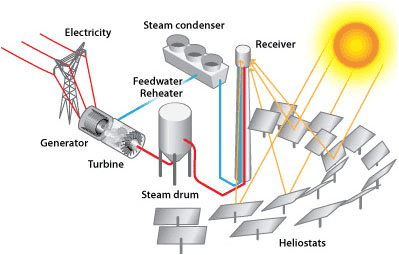
\includegraphics[width=0.6\linewidth]{FIG/power_tower}
\caption[Schematic CR power plant concept.]{Schematic CR power plant concept \cite{U.S.DOE2013}.}\label{power_tower}
\end{figure}


\begin{figure}[htbp]  
\centering
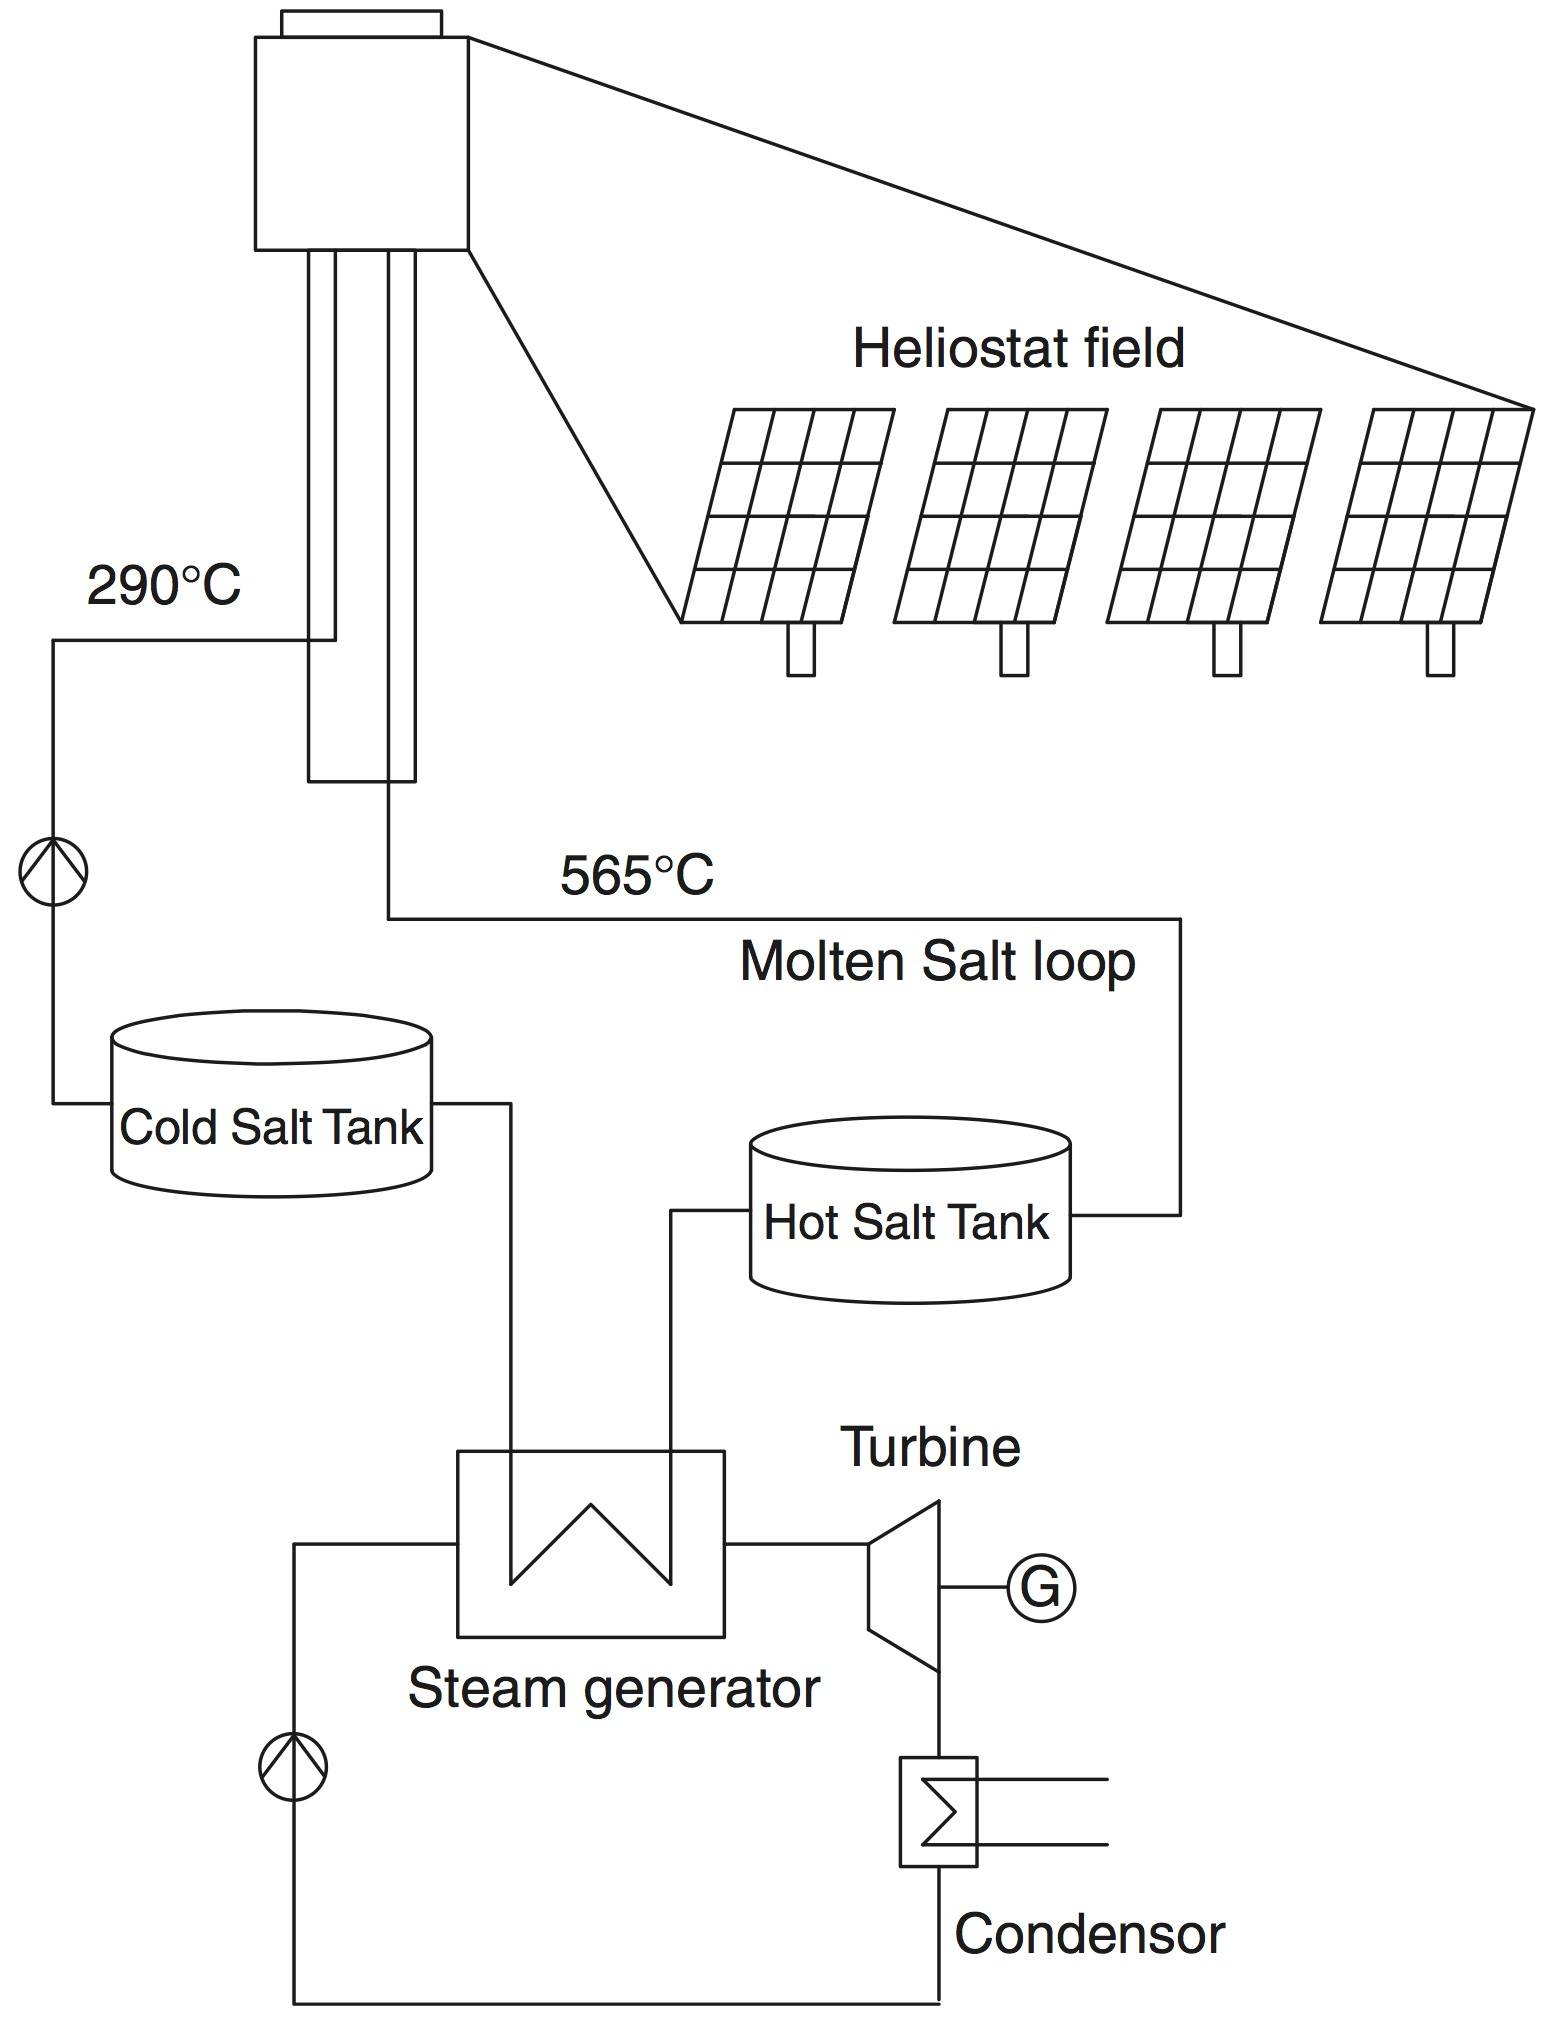
\includegraphics[width=0.45\linewidth]{FIG/towerdirecttwotank}
\caption[Simplified scheme of \emph{Solar Two} CRS power plant with direct storage of molten salt used as heat transfer fluid.]{Simplified scheme of \emph{Solar Two} CRS power plant with direct storage of molten salt used as heat transfer fluid \cite{Richter2013}.}\label{towerdirecttwotank}
\end{figure}

\pagebreak
\subsection{Parabolic-trough concentrating solar power} \label{subsection_PTC}


\begin{figure}[htbp] 
\centering
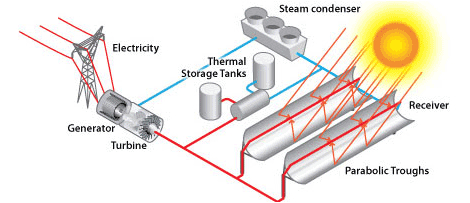
\includegraphics[width=0.7\linewidth]{FIG/parabolic_troughs}
\caption[Schematic parabolic trough power plant concept.]{Schematic parabolic trough power plant concept \cite{U.S.DOE2013}.}\label{parabolic_troughs}
\end{figure}

\begin{figure}[htbp] 
\centering
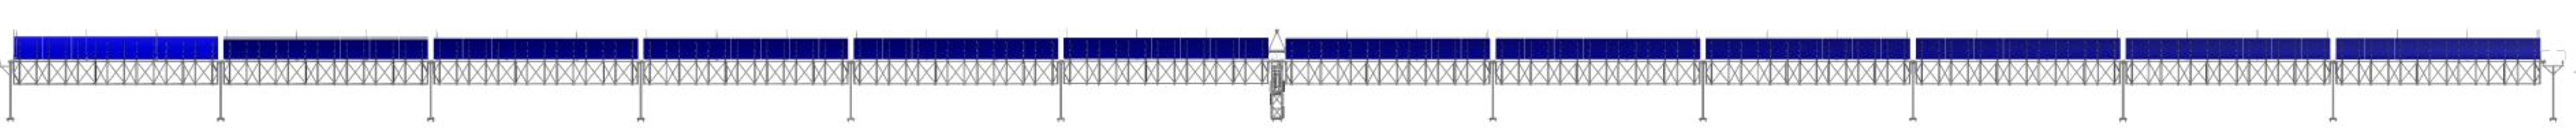
\includegraphics[width=1\linewidth]{FIG/SCA_EuroTrough}
\caption[Solar Collector Assembly (SCA) composed of 12 EuroTrough collector elements (SCE).]{Solar Collector Assembly (SCA) composed of 12 EuroTrough collector elements (SCE) \cite{VonReeken2014}.}\label{SCA_EuroTrough}
\end{figure}

\pagebreak
\begin{figure}[htbp] 
\centering
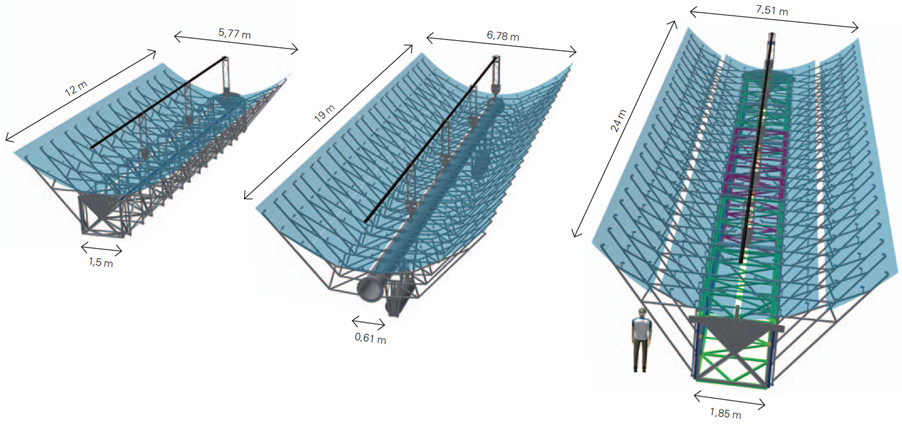
\includegraphics[width=1\linewidth]{FIG/Kollektoren}
\caption[Evolution of parabolic trough collector sizes over 3 development cycles (Eurotrough, HelioTrough, Ultimate Trough).]{Evolution of parabolic trough collector sizes over 3 development cycles (Eurotrough, HelioTrough, Ultimate Trough)\cite{Schlaichbergermannundpartner}.}\label{Kollektoren}
\end{figure}


\begin{figure}[htbp]  
\centering
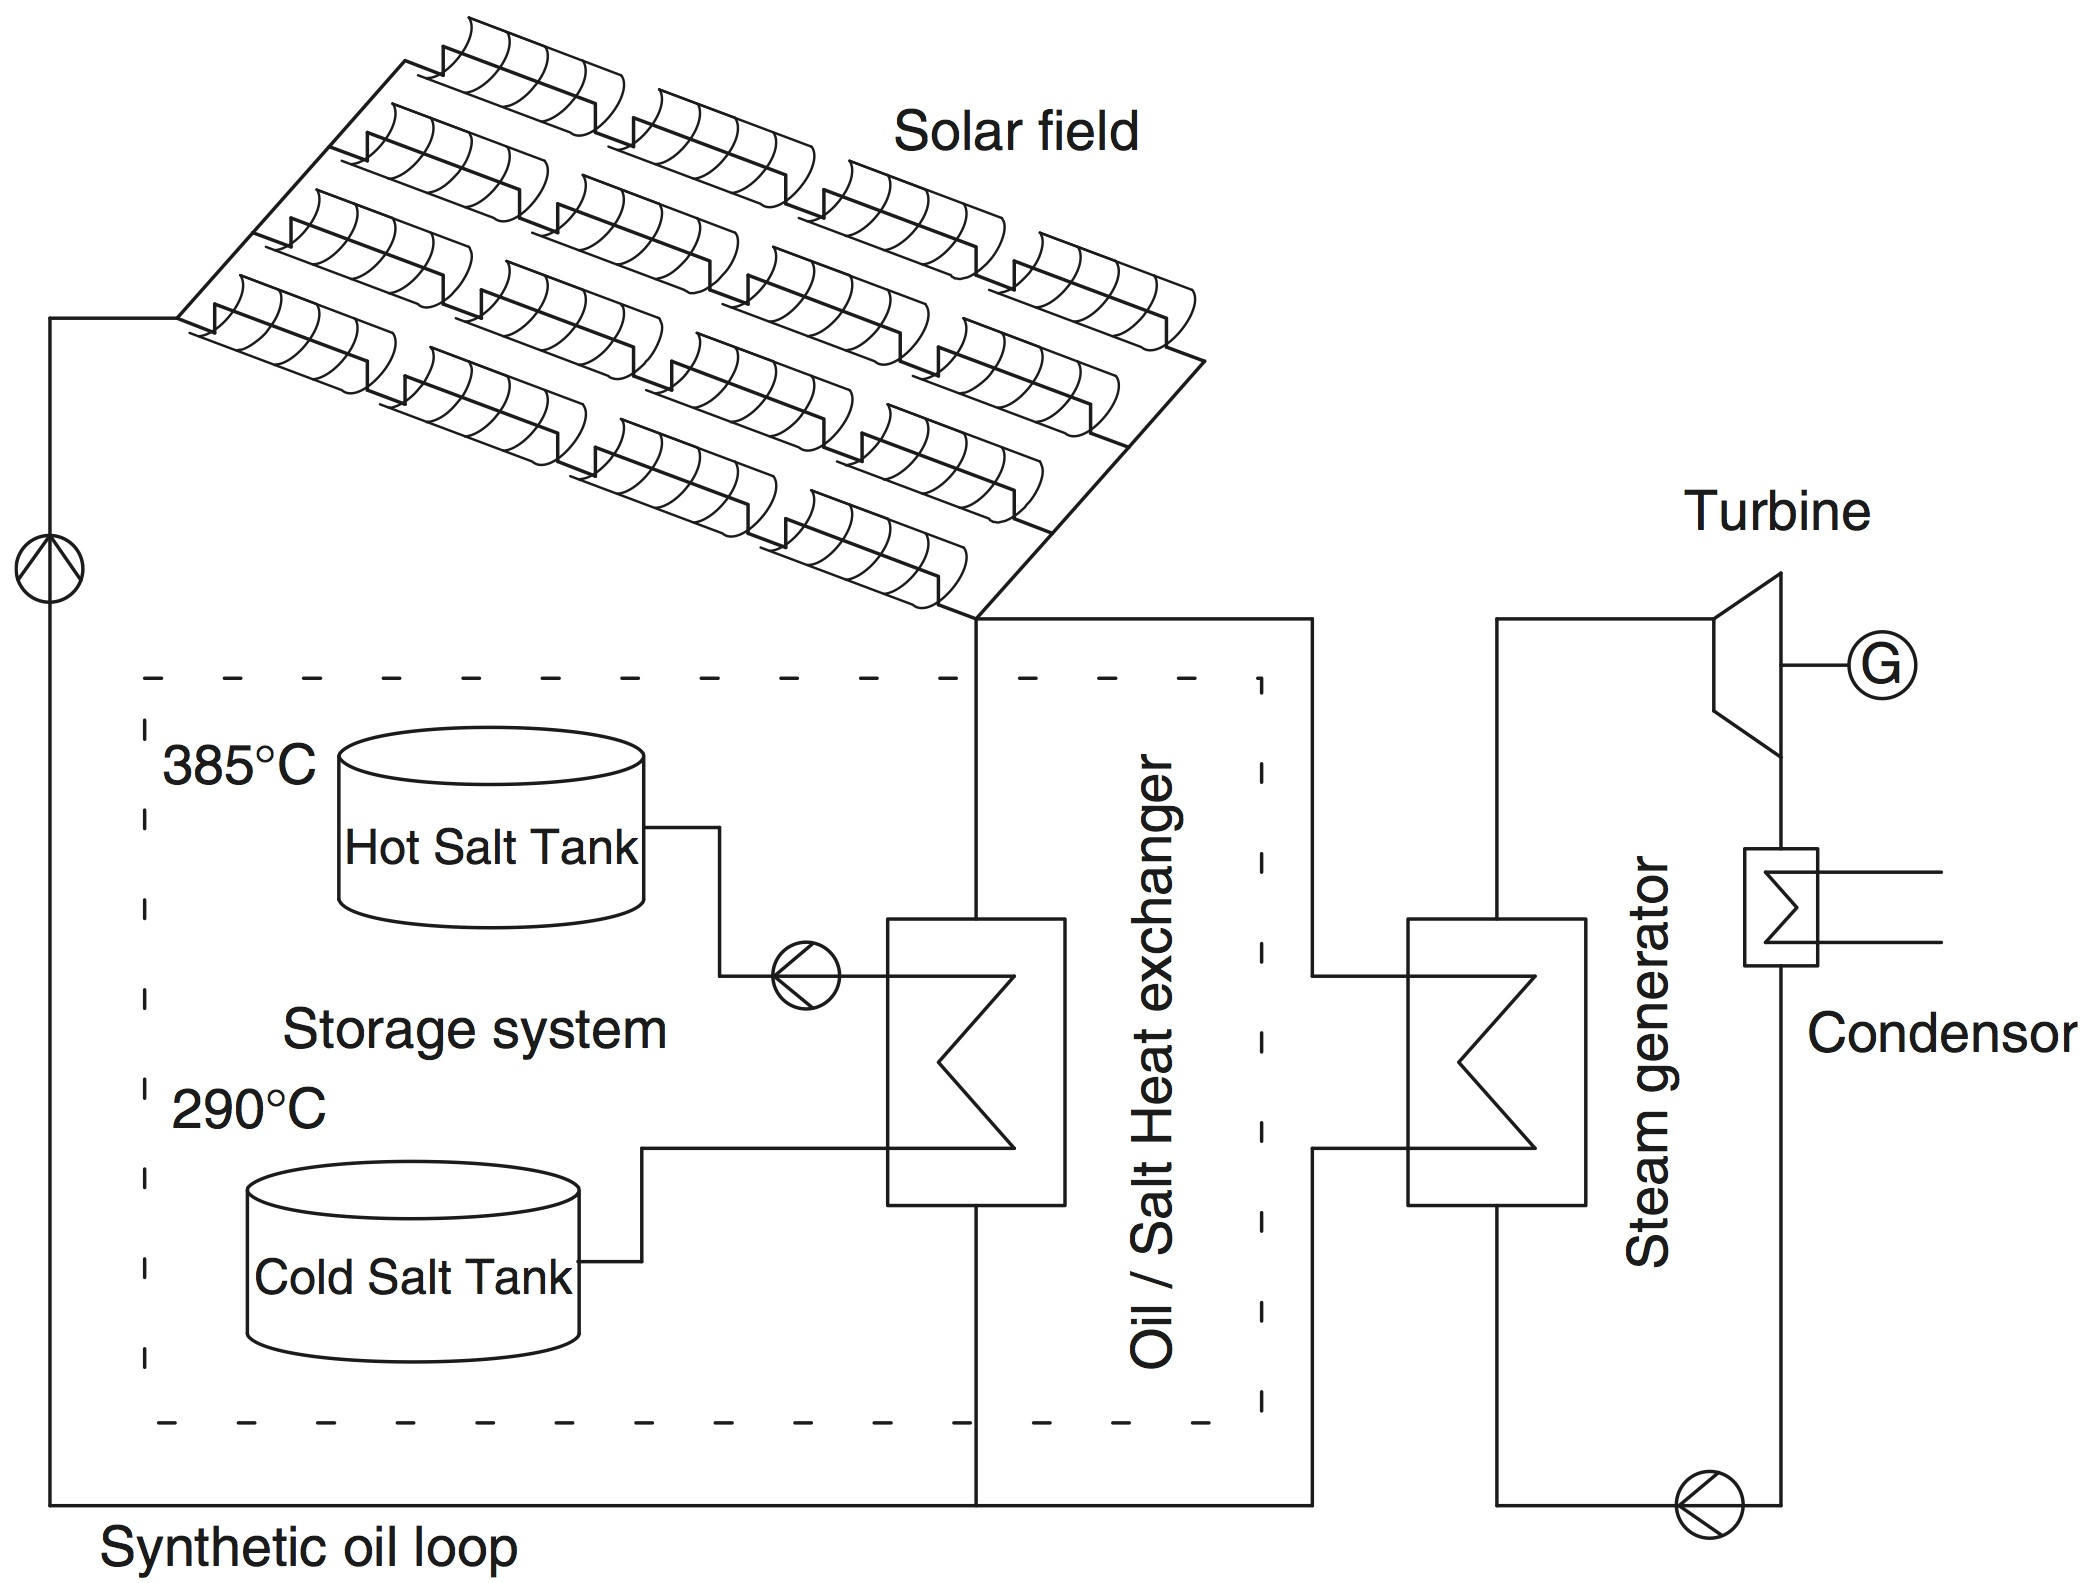
\includegraphics[width=0.45\linewidth]{FIG/troughtindirecttwotank}
\caption[Simplified scheme of PTC power plant with indirect storage system using molten salt.]{Simplified scheme of PTC power plant with indirect storage system using molten salt \cite{Steinmann2012}.}\label{troughtindirecttwotank}
\end{figure}

\pagebreak
\section{Large scale PV power plants}\label{Large scale photo voltaic (PV) power plants}
two axis tracking PV
\subsection{Large-scale PV power plants}

\subsection{Large-scale electrical energy storage systems}
electrical energy storage (EES)
EESSchema
\begin{figure}[htbp]  
\centering
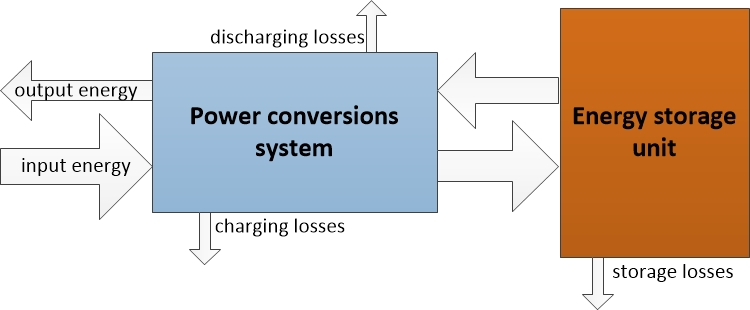
\includegraphics[width=0.65\linewidth]{FIG/EESSchema}
\caption[Schema of an electrical energy storage (EES) system and there energy losses.]{Schema of an electrical energy storage (EES) system and there energy losses.}\label{TCC_EES}
\end{figure}

\begin{equation}
\textrm{Overall storage efficiency (AC-to-AC)} =\frac{E_{out} \textrm{ (kWh)} }{E_{in} \textrm{ (kWh)}}
\end{equation}

\begin{figure}[htbp]  
\centering
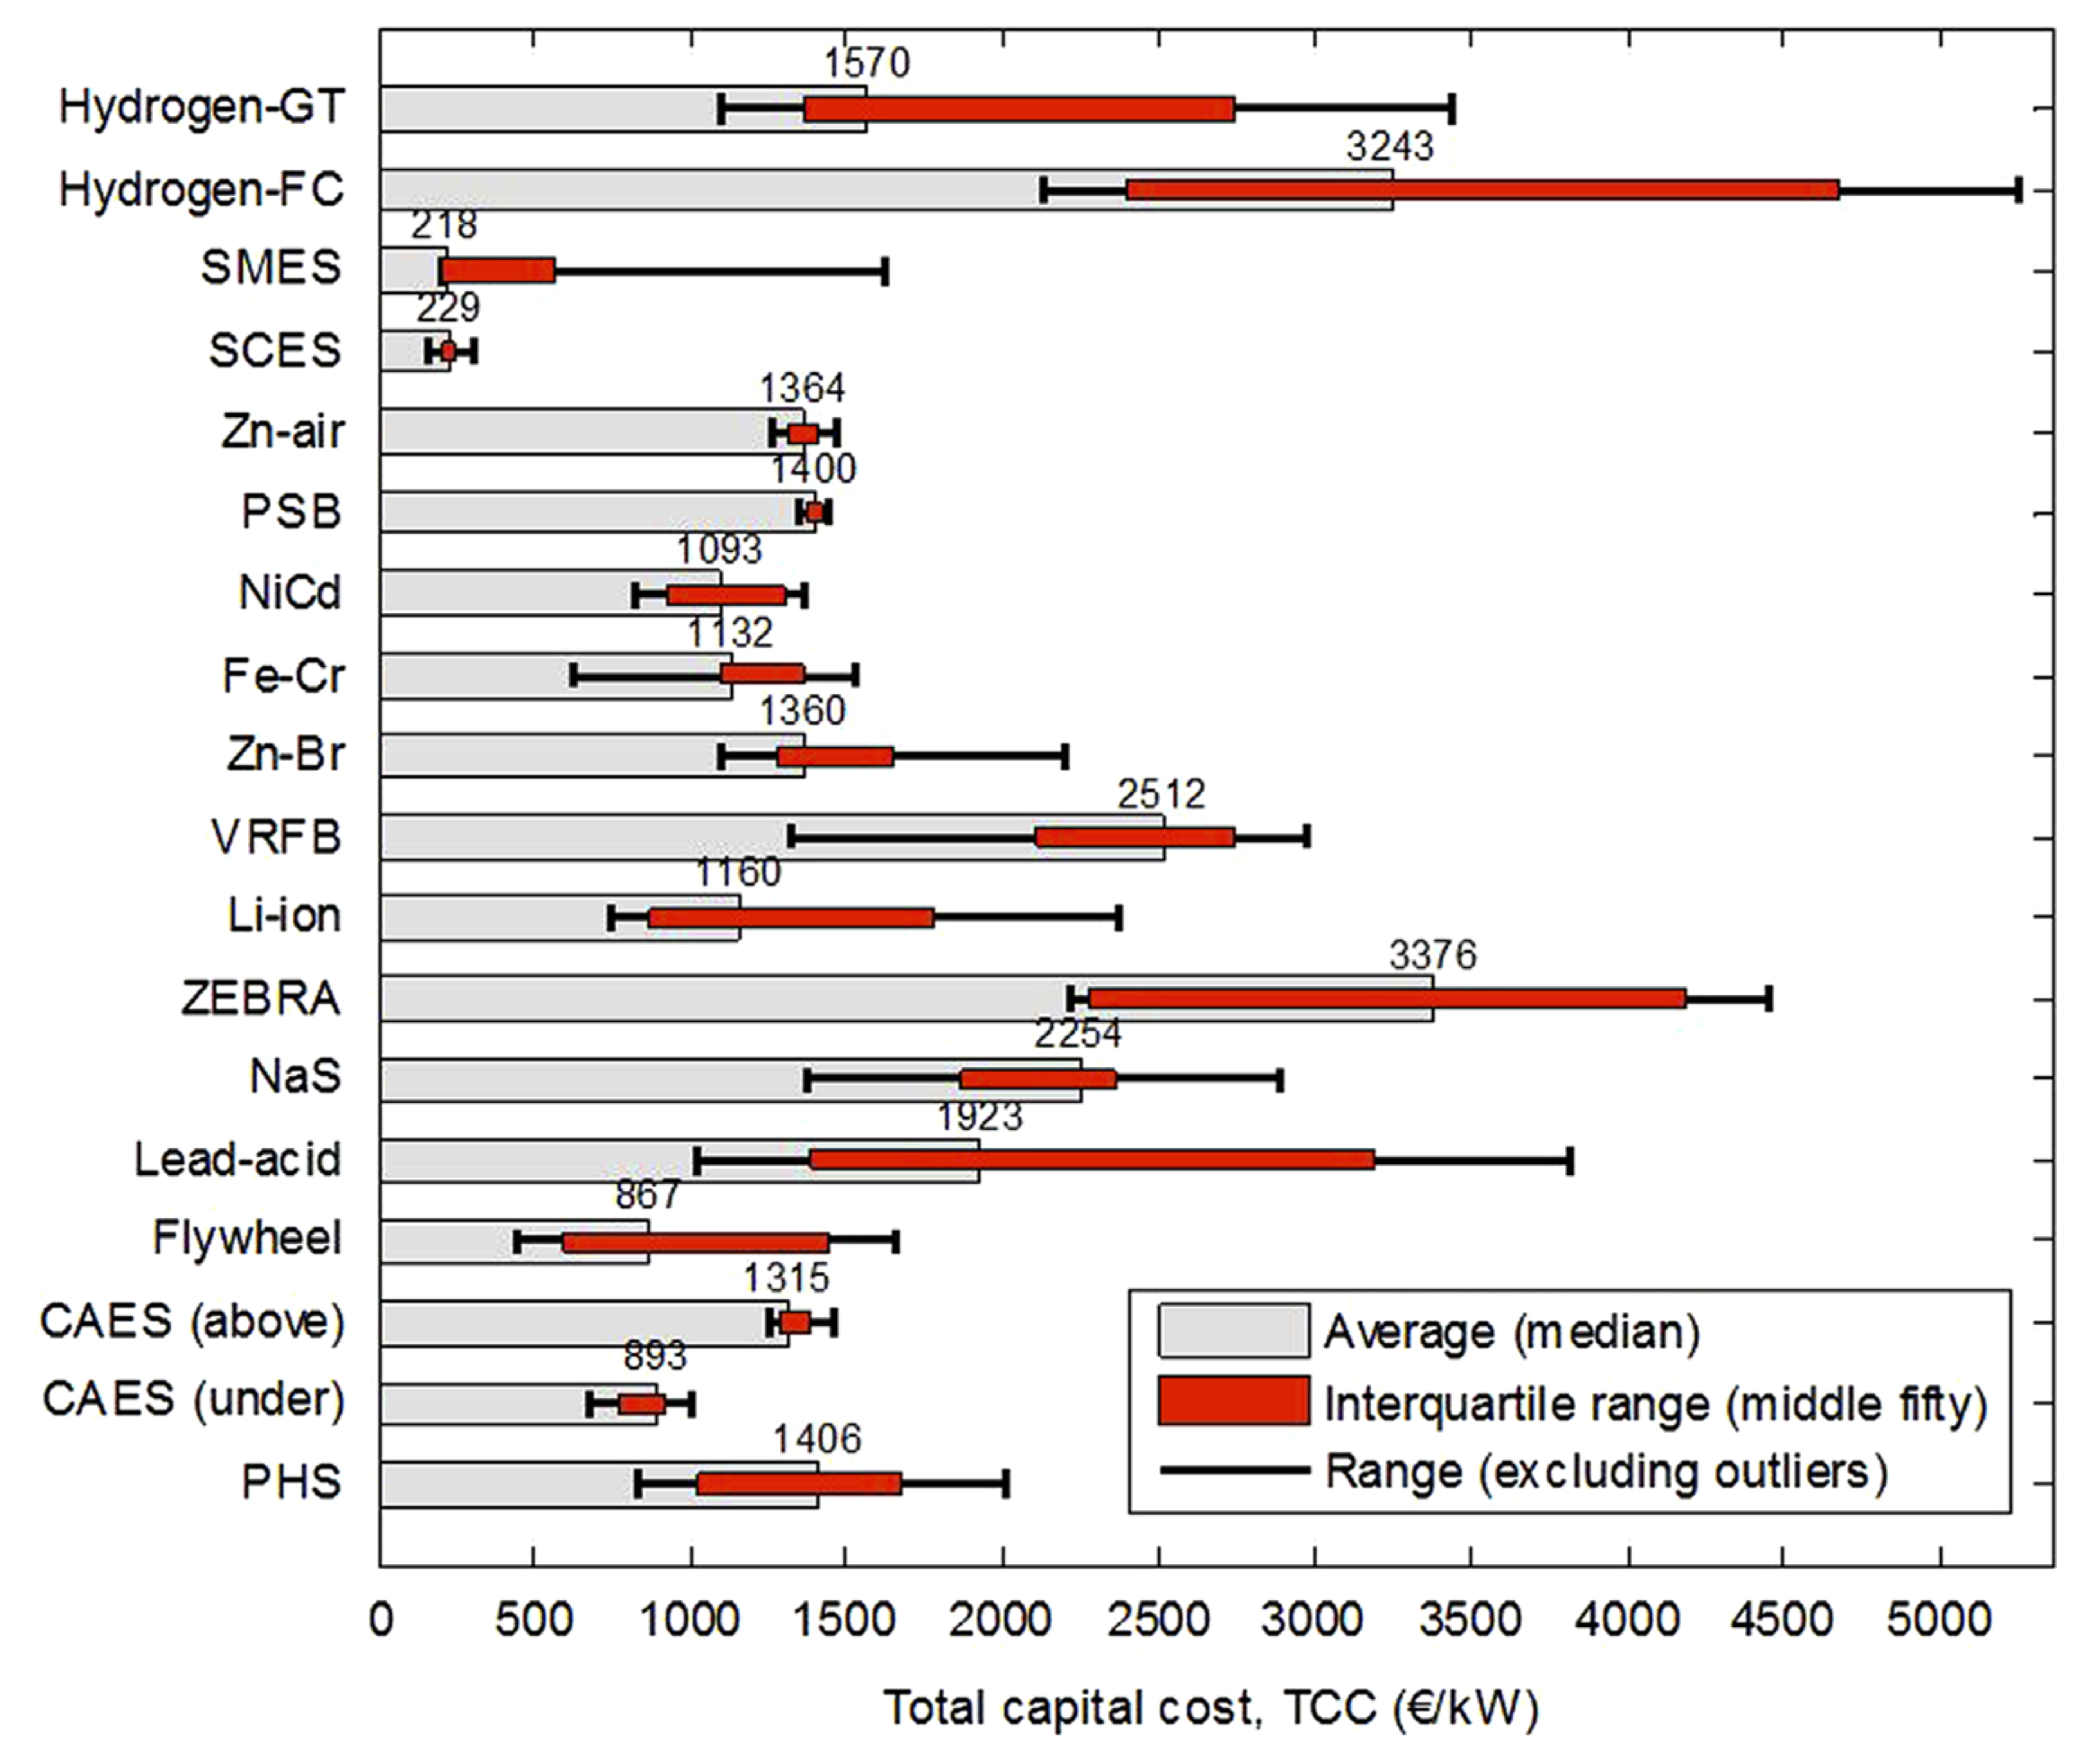
\includegraphics[width=0.75\linewidth]{FIG/TCC_EES}
\caption[Total capital cost in Euro (€) of large-scale EES systems per unit of nominal power rating including costs of power electronics, storage part, fixed obtain and maintainence and maybe incidental replacement costs.]{Total capital cost in Euro (€) of large-scale EES systems per unit of nominal power rating including costs of power electronics, storage part, fixed obtain and maintainence and maybe incidental replacement costs \cite{Zakeri2015}.}\label{TCC_EES}
\end{figure}